%\documentclass[mathserif]{beamer}
\documentclass[handout]{beamer}
%\usetheme{Goettingen}
\usetheme{Warsaw}
%\usetheme{Singapore}
%\usetheme{Frankfurt}
%\usetheme{Copenhagen}
%\usetheme{Szeged}
%\usetheme{Montpellier}
%\usetheme{CambridgeUS}
%\usecolortheme{}
%\setbeamercovered{transparent}
\usepackage[english, activeacute]{babel}
\usepackage[utf8]{inputenc}
\usepackage{amsmath, amssymb}
\usepackage{dsfont}
\usepackage{graphics}
\usepackage{cases}
\usepackage{graphicx}
\usepackage{pgf}
\usepackage{epsfig}
\usepackage{amssymb}
\usepackage{multirow}	
\usepackage{amstext}
\usepackage[ruled,vlined,lined]{algorithm2e}
\usepackage{amsmath}
\usepackage{epic}
\usepackage{epsfig}
\usepackage{fontenc}
\usepackage{framed,color}
\usepackage{palatino, url, multicol}
\usepackage{listings}
%\algsetup{indent=2em}


\vspace{-0.5cm}
\title{Directed Graphical Models}
\vspace{-0.5cm}
\author[Felipe Bravo Márquez]{\footnotesize
%\author{\footnotesize  
 \textcolor[rgb]{0.00,0.00,1.00}{Felipe José Bravo Márquez}} 
\date{ \today }




\begin{document}
\begin{frame}
\titlepage


\end{frame}


%%%%%%%%%%%%%%%%%%%%%%%%%%%


\begin{frame}{Directed Graphical Models}
\scriptsize{
\begin{itemize}
\item Probabilistic graphical models (PGMs) are a rich framework for encoding probability distributions over complex domains  \cite{koller2009probabilistic}.

\item In this class we will focus on directed graphical models (DGMs), which are one type of PGM.

\item Directed graphical models (DGMs) are a family of probability distributions that admit a compact parametrization that can be naturally described using a \textbf{directed graph}.

\item DGMs are also known as \textbf{Bayesian networks}.

\item We won't use that term in this class because statistical inference for DGMs can be performed using frequentist or Bayesian methods \cite{wasserman2013all}.

\item These types of graphs are also called \textbf{causal graphs} or \textbf{causal diagrams}.

 
\end{itemize}



} 

\end{frame}


\begin{frame}{Directed Graphical Models}
\scriptsize{
\begin{itemize}
\item DGMs link two very different branches of mathematics: probability and graph theory. 

\item They also have intriguing connections to philosophy, particularly the question of \textbf{causality}.

\item At the same time, they are widely used in statistics and machine learning.

\item DGMs can be used to solve problems in fields as diverse as medicine, language processing, vision, and many others \cite{ermon_kuleshov}. 

\item But before introducing them more formally we need to learn the following mathematical concepts:

\begin{enumerate}
\scriptsize{
 \item Conditional independence
 \item The chain rule of probability
 \item Directed acyclical graphs }
\end{enumerate}

 
\end{itemize}



} 

\end{frame}



\begin{frame}{Conditional Independence}
\scriptsize{
\begin{itemize}

\item Two random variables $X$ and $Y$ are independent, written $X \perp Y$ if $f(x,y)=f(x)f(y)$ for all values of $x$, $y$.


\item This also implies that $f(x|y)=f(x)$ and $f(y|x)=f(y)$.


\item Notice that $f$ can be either a density function for continous random variables or a probability mass function for discrete random variables.

\item In the same way  $f(x|y)$ and $f(y|x)$ correspond to conditional densities or mass functions. 

\item Now, suppose we have three random variables $A,B,C$. 

\item $A$ and $B$ are conditionally independent given $C$, written $A \perp B | C$, if:

\begin{displaymath}
f(a|b,c) = f(a|c)
\end{displaymath}


for all a, b and c.


 
\end{itemize}




} 

\end{frame}



\begin{frame}{Conditional Independence}
\scriptsize{

\begin{itemize}
 \item Intuitively, $A \perp B | C$ means that, once you know $C$, $B$ provides no extra information about $A$.

\item Notice that $A \perp B | C$ doesn't necessarily imply that $A \perp B$.
 
\end{itemize}



\begin{block}{Example}
\begin{itemize}
 \item Let $H,V,A$ be three random variables representing a person's height, vocabulary and age.
 \item H and V are dependent $f(v|h) \neq f(v)$ 
 since very small people tend to be children, known for their more basic vocabularies. 
 \item But knowing that two people are 19 years old (i.e., conditional on age) there is no reason to think that one person's vocabulary is larger if we are told that they are taller: 
 \begin{displaymath}
 f(v|h,a)=f(v|a) \Leftrightarrow V \perp H | A 
 \end{displaymath}

\end{itemize}


\end{block}





} 

\end{frame}


\begin{frame}{The chain rule of probability}
\scriptsize{
\begin{itemize}

\item For a set of random variables $X_1,\dots, X_n$, the chain rule of probability allow us to express the joint probability function $f(x_1,x_2,\dots, x_n)$ as a product of $n$ conditional probabilities:



\begin{displaymath}
f(x_1,x_2,\dots,x_n)=f(x_1)f(x_2|x_1)f(x_3|x_2,x_1)\dots f(x_n|x_{n-1},\dots,x_2,x_1).
 \end{displaymath}

\item For example for the case of $n=3$

\begin{displaymath}
f(x_1,x_2,x_3)=f(x_1)f(x_2|x_1)f(x_3|x_2,x_1)
 \end{displaymath}

using the definition of conditional probabilities we have that


\begin{displaymath}
 f(x_2|x_1) = f(x_1,x_2)/f(x_1)
\end{displaymath}

 and \begin{displaymath}
f(x_3|x_2,x_1)=f(x_1,x_2,x_3)/f(x_1,x_2)       
     \end{displaymath}

\item By replacing these expressions into the chain of products, many expressions cancel out and we obtain $f(x_1,x_2,x_3)$.     

\end{itemize}



} 

\end{frame}


\begin{frame}{Joint Probabilities}
\scriptsize{
\begin{itemize}

\item Expressing a joint probability function can be expensive.

\item For example if there are $m$ binary random variables, the complete distribution is specificied by $2^{m}-1$ joint probabilities.

\item For example, if we have two Boolean variables $(A,B)$, we need the probabilities $\mathbb{P}(A,B)$, $\mathbb{P}(\neg A,B)$, $\mathbb{P}(A,\neg B)$, and $\mathbb{P}(\neg A, \neg B)$.

\item A joint distribution for a set of random variables gives all the information there is about the distribution.


\item Note that for $m$ boolean variables, the joint distribution contains $2^m$ values. 

\item However, the sum of all the joint probabilities must be 1 because the probability of all possible outcomes must be 1. 

\item Thus, to specify the joint distribution, one needs to specify $2^{m-1}$ numbers.


\end{itemize}



} 

\end{frame}


\begin{frame}{Joint Probabilities}
\scriptsize{
\begin{itemize}



\item The main idea of DGMs is that by assuming that some variables are conditionally independent we can use the probability chain rule to represent the joint distribution more compactly.

\item For example in the previous example, a conditional independence assumption could be: $X_3 \perp X_2| X_1$: $f(x_3|x_2,x_1)= f(x_3|x_2)$.

\item Then our joint distribution would be reduced to:

\begin{displaymath}
f(x_1,x_2,x_3)=f(x_1)f(x_2|x_1)f(x_3|x_2)
 \end{displaymath}

 
\item In the following slides we will try to explain these ideas with an example taken from \cite{koller2009probabilistic}. 

\end{itemize}



} 

\end{frame}

\begin{frame}{Example}
\scriptsize{
\begin{itemize}


\item Consider the problem faced by a company trying to hire a recent college graduate. 
\item The company's goal is to hire intelligent employees, but there is no way to test intelligence directly. 

\item However, the company has access to the student's SAT scores\footnote{The SAT is a standardized test widely used for college admissions in the United States.}, which are informative but not fully indicative. 

\item Thus, our probability space is induced by the two random variables Intelligence (I) and SAT (S). 
\item For simplicity, we assume that each of these takes two values: $Val(I) = \{i_1 , i_0 \}$, which represent
the values high intelligence ($i_1$ ) and low intelligence $(i_0)$.
\item Similarly $Val(S) = \{s_1 , s_0 \}$, which
also represent the values high (score) and low (score), respectively.

\end{itemize}



} 

\end{frame}


\begin{frame}{Example}
\scriptsize{
\begin{itemize}

\item Thus, our joint distribution in this case has four entries. 
\item For example, one possible joint distribution f would be:

\begin{table}
\centering
  \begin{tabular}{cc|c} \hline
$I$ & $S$ & $f(I,S)$  \\ \hline
$i^0$ & $s^0$ & 0.665 \\
$i^0$ & $s^1$ & 0.035 \\
$i^1$ & $s^0$ & 0.06 \\
$i^1$ & $s^1$ & 0.24 
\end{tabular} 
\end{table}

\item Using the chain rule of conditional probabilities, we have that

\begin{displaymath}
 f(I,S) = f(I)f(S|I)
\end{displaymath}
\item Intuitively, we are representing the process in a way that is more compatible with causality.

\item Various factors (e.g., genetics, upbringing) first determined (stochastically) the student's intelligence.
\item Her performance on the SAT is determined (stochastically) by his intelligence. 
\item We note that the models we construct are not required to follow causal intuitions, but they often do.



\end{itemize}



} 

\end{frame}


\begin{frame}{Directed Acyclic Graphs (DAGs)}
\scriptsize{
\begin{itemize}
\item A directed graph consists of a set of nodes with arrows between some nodes.


\item Graphs are useful for representing independence relations between variables.

\item More formally, a directed graph G consists of a set of vertices V and an edge set E of ordered pairs of
vertices.

\item For our purposes, each vertex corresponds to a random variable. 

\item If $(Y, X) \in E$  then there is an arrow pointing from Y to X. 

\begin{figure}[h!]
	\centering
	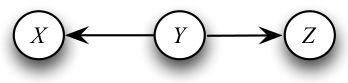
\includegraphics[scale=0.5]{pics/dag1.png}
	\caption{A directed graph with vertices $V = \{X, Y, Z\}$ and edges $E = \{(Y, X), (Y, Z)\}$.}
	\end{figure} 


 
\end{itemize}



} 

\end{frame}



\begin{frame}{Directed Acyclic Graphs (DAGs)}
\scriptsize{
\begin{itemize}
\item If an arrow connects two variables X and Y (in either direction) we say that X and Y are adjacent.


\item If there is an arrow from X to Y then X is a parent of Y and Y is a child of X.

\item The set of all parents of X is denoted by $\pi_{X}$ or $\pi(X)$.

\item A directed path between two variables is a set of arrows all pointing in the same direction linking one variable to the
other such as the chain shown below:

\begin{figure}[h!]
	\centering
	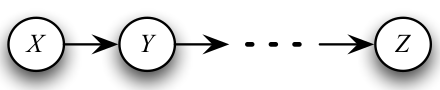
\includegraphics[scale=0.5]{pics/dag2.png}
	\caption{A chain graph with a directed path.}
	\end{figure} 

\item X is an ancestor of Y if there is a directed path from X to Y (or X = Y ).

\item We also say that Y is a descendant of X.
 
\end{itemize}



} 

\end{frame}

\begin{frame}{Directed Acyclic Graphs (DAGs)}
\scriptsize{
\begin{itemize}
\item A directed path that starts and ends at the same variable is called a cycle.

\item A directed graph is acyclic if it has no cycles. 

\item In this case we say that the graph is a directed
acyclic graph or DAG. 


\begin{figure}[h!]
	\centering
	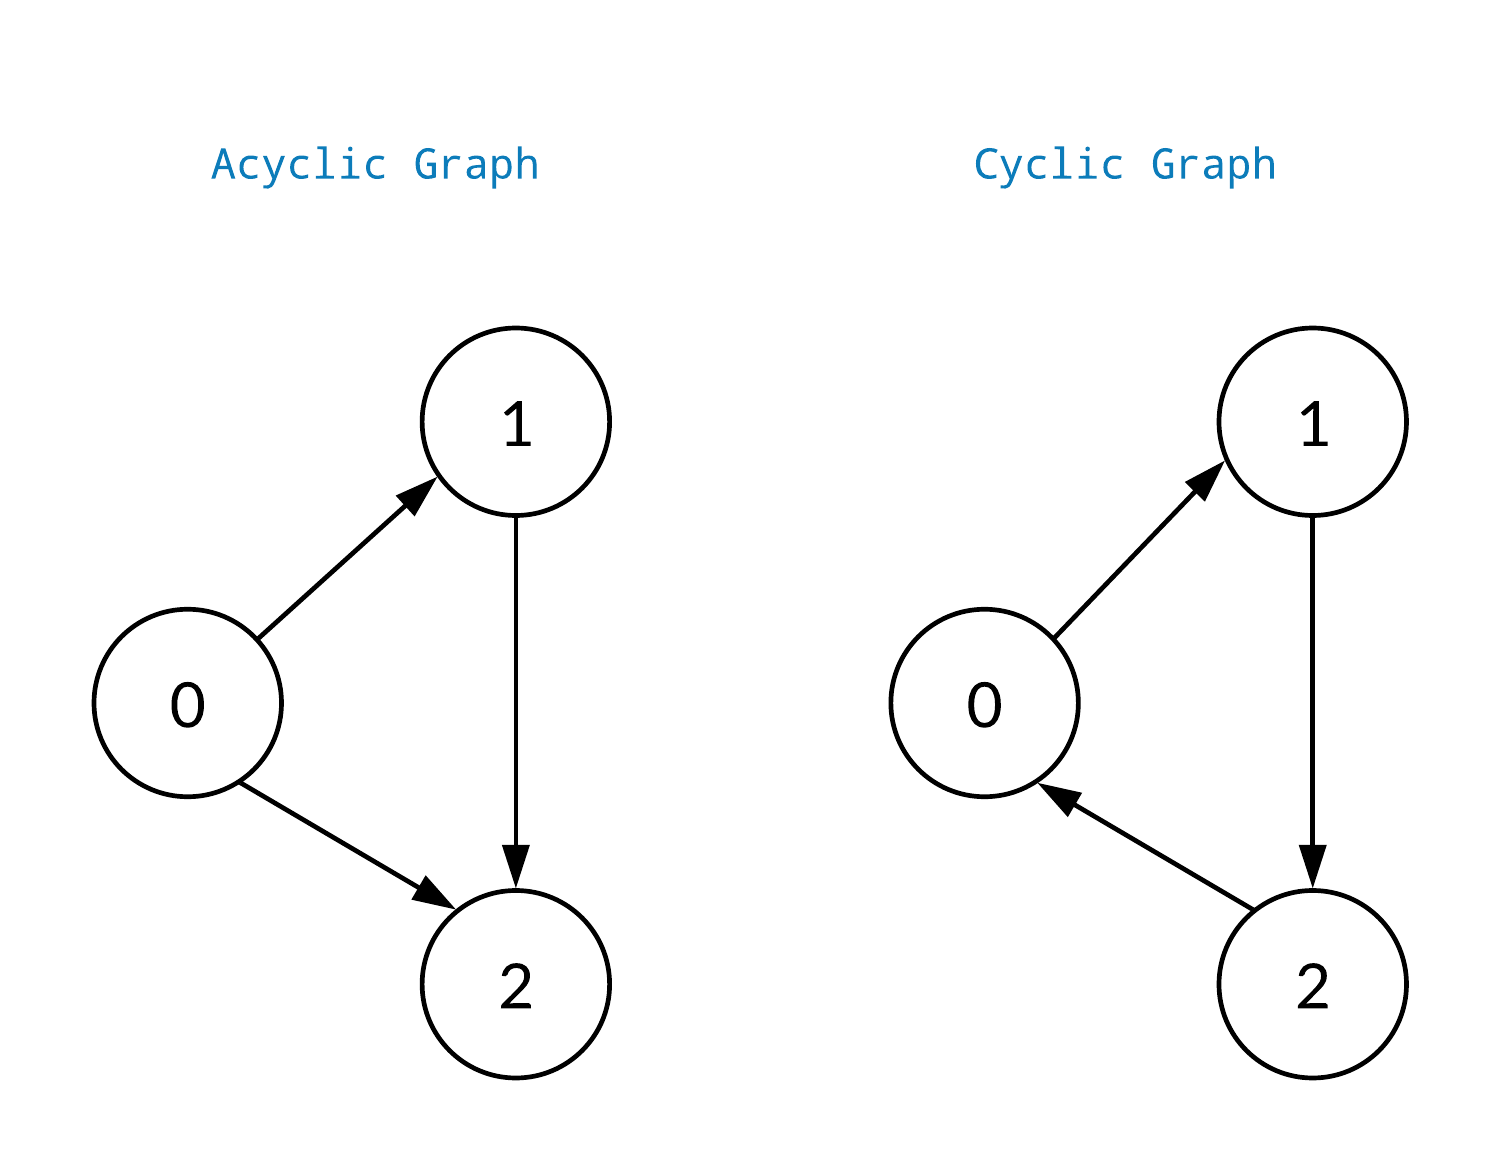
\includegraphics[scale=0.12]{pics/cycle.png}
	\end{figure} 



\item From now on, we only deal with directed acyclic graphs since it is very difficult to provide a coherent probability semantics over graphs with directed cycles.
 
 
 
\end{itemize}



} 

\end{frame}


\begin{frame}{Probability and DAGs}
\scriptsize{
\begin{itemize}

\item For the remainder of this class we will use the terms   directed graphical model (DGM) and directed acyclical graph (DAG) interchangeably. 

\item A DAG is a distribution in which each factor on the right hand side depends only on a small number of ancestor variables $\pi(x)$. \cite{ermon_kuleshov}



\item Let $G$ be a DAG with vertices $V = (X_1 , \dots , X_d )$. 

\item If $P$ is a distribution for $V$ with probability function $f(x)$ (density or masss), we say that $G$ represents $P$ , if

\begin{displaymath}
 f(x) = \prod_{j=1}^d f(x_j| \pi_{x_j})
\end{displaymath}

where $\pi_{x_j}$ is the set of parent nodes of $X_j$



\end{itemize}



} 

\end{frame}

\begin{frame}{Probability and DAGs}
\scriptsize{
\begin{itemize}


\item The next figure shows a DAG with four variables.

\begin{figure}[h!]
	\centering
	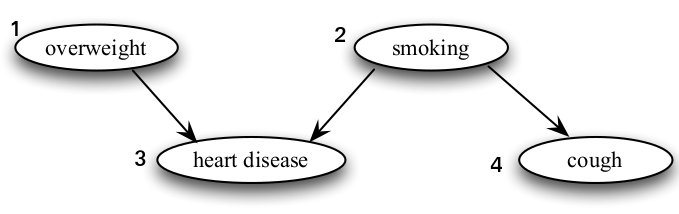
\includegraphics[scale=0.4]{pics/dag3.png}
	\end{figure} 



\item The probability function takes the following decomposition:

\item $f($overweight, smoking, heart disease, cough$) =$ \\    $f($overweight$) \times f($smoking$) \times f($heart, disease$|$ overweight, smoking$) \times f($cough$|$smoking$)$. 


\end{itemize}



} 

\end{frame}


\begin{frame}{Causal DAGs}
\scriptsize{
\begin{itemize}


\item The interpretation of direct acyclic graphs as carriers of independence assumptions does not necessarily imply causation.

\item In fact, it will be valid for any set of recursive independencies along any ordering of the variables, not necessarily causal or chronological.

\item However, the ubiquity of DAG models in statistical and AI applications stems (often unwittingly) primarily from their causal interpretation 

\item That is, as a system of processes, one per family, that could account for the generation of the observed data. 

\item It is this causal interpretation that explains why DAG models are rarely used in any variable ordering other than those which respect the direction of time and causation. \cite{pearl2009causality}

\end{itemize}



} 

\end{frame}





\begin{frame}{An Example}
\scriptsize{
\begin{itemize}
\item The best way to understand DAGs is to imagine trying to model a situation in which causality plays a role.
\item And also our understanding of what is actually going on is
incomplete
\item So we need to describe things probabilistically. 

\item The following example is based on \cite{charniak1991bayesian}.

\item Eugene Charniak is a famous AI researcher who's got the following situation.

\item When he goes home at night, he wants to know if his family is home before trying the doors. 

\item Often when his wife leaves the house, she turns on an outdoor light. 

 
\end{itemize}



} 

\end{frame}



\begin{frame}{An Example}
\scriptsize{
\begin{itemize}

\item Eugene's wife can also turn on the outdoor light if she is expecting a guest.

\item Also, they have a female dog. 

\item When nobody is home, the dog is put in the back yard. 

\item The same is true if the dog has bowel troubles. 

\item Finally, if the dog is in the backyard, Eugene's will probably hear her barking 

\item The next slide shows a DAG encoding all the above causal relationships.

 
\end{itemize}



} 

\end{frame}


\begin{frame}{An Example}
\scriptsize{

\begin{figure}[h!]
	\centering
	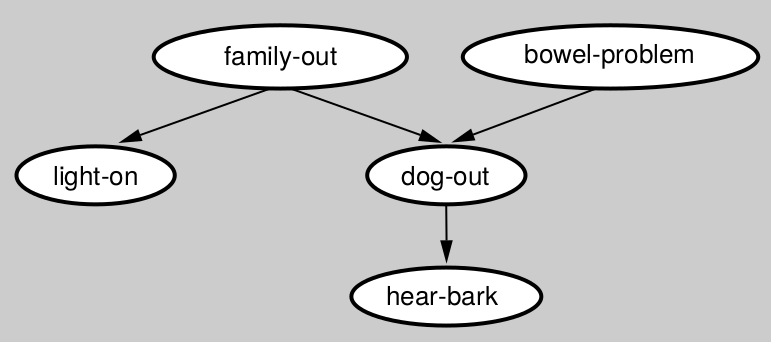
\includegraphics[scale=0.4]{pics/fodag.png}
	\end{figure} 

\begin{itemize}

\item The DAG can help to predict what will happen in a particular scenario (if his family goes out, the dog goes out) 
\item Or to infer causes from observed effects (if the light is on and the dog is out, then his family is probably out).



 
\end{itemize}



} 

\end{frame}


\begin{frame}{D-separation}
\scriptsize{
\begin{itemize}
\item sdsad

 
\end{itemize}



} 

\end{frame}


\begin{frame}{Plate Notation}
\scriptsize{
\begin{itemize}
\item sdsad

 
\end{itemize}



} 

\end{frame}



\begin{frame}{Estimation for DAGs}
\scriptsize{
\begin{itemize}
\item Two estimation questions arise in the context of DAGs. 
\item First, given a DAG $\mathcal{G}$ and data $d_1,\dots,d_n$ from a distribution $f$ consistent with $\mathcal{G}$, how do we estimate f?

\item Second, given data $d_1,\dots,d_n$ how do we estimate $\mathcal{G}$?

\item The first question is pure estimation while the second involves model selection.

\item These are very involved topics and are beyond the scope of this course.

\item We will just briefly mention the main ideas.

 
\end{itemize}



} 

\end{frame}


\begin{frame}{Estimation for DAGs}
\scriptsize{
\begin{itemize}

\item If we are doing frequentist inference, we typically use some parametric model $f(x|\pi_x;\theta_x)$ for each conditional density. 

\item The likelihood function is then

\begin{displaymath}
 \mathcal{L}(\theta) = \prod_{i=1}^nf(d_i;\theta) ) =  \prod_{i=1}^n\prod_{j=1}^mf(X_{ij}|\pi_j;\theta_j) 
\end{displaymath}

\item where $X_{ij}$ is the value of $X_j$ for the ith data point and j are the parameters for the-jth conditional density. 

\item We can then estimate the parameters by maximum likelihood.

\item On the other hand, if we want to perform Bayesian inference we must set priors for all our variables $X_1,\dots,X_m$ and estimate the posterior accordingly.

 
\end{itemize}



} 

\end{frame}

\begin{frame}{Estimation for DAGs}
\scriptsize{
\begin{itemize}

\item To estimate the structure of the DAG itself, we could fit every possible DAG
using maximum likelihood and use AIC (or some other method) to choose a
DAG. 

\item However, there are many possible DAGs so we would need much data
for such a method to be reliable.

\item Also, searching through all possible DAGs is a serious computational challenge. 

\item Producing a valid, accurate confidence set for the DAG structure would require astronomical sample sizes. 

\item If prior information is available about part of the DAG structure, the computational and statistical problems are at least partly ameliorated \cite{wasserman2013all}.

 
\end{itemize}



} 

\end{frame}


\begin{frame}{Conclusions}
\scriptsize{

\begin{itemize}
\item Blabla
\end{itemize}


} 
\end{frame}


%%%%%%%%%%%%%%%%%%%%%%%%%%%
\begin{frame}[allowframebreaks]\scriptsize
\frametitle{References}
\bibliography{bio}
\bibliographystyle{apalike}
%\bibliographystyle{flexbib}
\end{frame}  









%%%%%%%%%%%%%%%%%%%%%%%%%%%

\end{document}
